\documentclass[11pt,a4paper]{article}
\usepackage[margin=1in, headheight=14pt]{geometry}
\usepackage{amsfonts,amsmath,amssymb,suetterl}
\usepackage{lmodern}
\usepackage[T1]{fontenc}
\usepackage{fancyhdr}
\usepackage{float}
\usepackage[utf8]{inputenc}
\usepackage{fontawesome}
\usepackage{enumerate}
\usepackage{xcolor}
\usepackage{hyperref}
\usepackage{tikz}
\usepackage{nicefrac}
\usepackage{subcaption}

\DeclareUnicodeCharacter{2212}{-}

\usepackage{mathrsfs}
\usepackage[nodisplayskipstretch]{setspace}

\setstretch{1.5}
\renewcommand{\footrulewidth}{0pt}

\parindent 0ex
\setlength{\parskip}{1em}
% \pagestyle{empty}

\begin{document}
    %
	\begin{center}
		\vspace*{8cm}
		\Huge MA202 –Differential Equations\\
		\LARGE LECTURE 12
  \end{center}
  \newpage
	%
  \section*{Linear systems of ODEs: Examples}
  \textbf{Example 1: Direction field (1 of 9)}
	\begin{itemize}
		\item Consider the homogeneous equation $x^\prime = Ax$ below.
		$$
		x^\prime =
		\begin{pmatrix}
			1 & 1\\
			4 & 1
		\end{pmatrix}x
		$$
		\item A direction field for this system is given below.
		\begin{figure}[H]
			\centering
				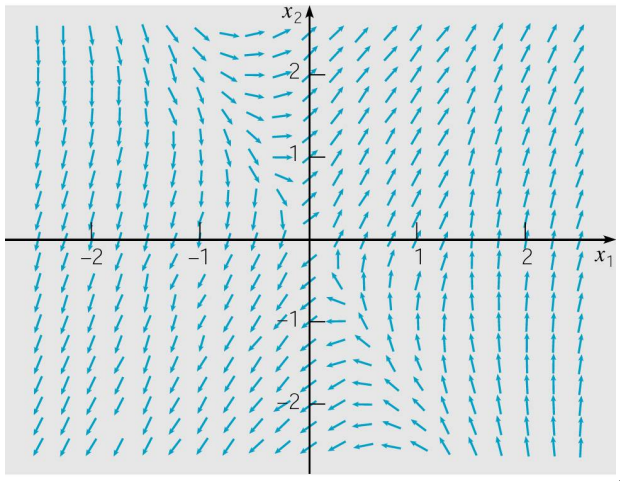
\includegraphics[width=0.45\textwidth]{figure/Lec12f1.PNG}
		\end{figure}
		\item Substituting $x = \xi e^{rt}$ in for $x$, and rewriting the system as $(A-rI)\xi=0$, we obtain
		$$
		\begin{pmatrix}
			1 - r & 1\\
			4 & 1-r
		\end{pmatrix}
		\begin{pmatrix}
			\xi_1\\
			\xi_2
		\end{pmatrix}
		=
		\begin{pmatrix}
			0\\
			0
		\end{pmatrix}
		$$
	\end{itemize}
	\textbf{Example 1: Eigenvalues (2 of 9)}
	\begin{itemize}
		\item Our solution has the form $x = \xi e^{rt}$, where $r$ and $\xi$ are found by solving
		$$
		\begin{pmatrix}
			1 - r & 1\\
			4 & 1-r
		\end{pmatrix}
		\begin{pmatrix}
			\xi_1\\
			\xi_2
		\end{pmatrix}
		=
		\begin{pmatrix}
			0\\
			0
		\end{pmatrix}
		$$
		\item Recalling that this is an eigenvalue problem, we determine $r$ by solving $\det(A-rI) = 0$:
		$$
		\begin{vmatrix}
			1 - r & 1\\
			4 & 1-r
		\end{vmatrix}
		= (1-r)^2-4
		= r^2-2r-3
		=(r-3)(r+1)
		$$
		\item Thus $r_1 = 3$ and $r_2 = -1$. We note that if one (or both) of the  off-diagonal terms of $A$ is $0$, the eigenvalues are just the  diagonal elements of $A$.
	\end{itemize}
	\textbf{Example 1: First eigenvector (3 of 9)}
	\begin{itemize}
		\item Eigenvector for $r_1 = 3$: Solve
		$$
		(A-rI)\xi = 0\ \Leftrightarrow \ 
		\begin{pmatrix}
			1-3 & 1\\
			4 & 1-3
		\end{pmatrix}
		\begin{pmatrix}
			\xi_1\\
			\xi_2
		\end{pmatrix}
		=
		\begin{pmatrix}
			0\\
			0
		\end{pmatrix}\ \Leftrightarrow\ 
		\begin{pmatrix}
			-2 & 1\\
			4 & -2
		\end{pmatrix}
		\begin{pmatrix}
			\xi_1\\
			\xi_2
		\end{pmatrix}
		=
		\begin{pmatrix}
			0\\
			0
		\end{pmatrix}
		$$
		by row reducing the augmented matrix:\\
		$
		\begin{pmatrix}
			-2 & 1 & 0\\
			4 & -2 & 0
		\end{pmatrix}\to
		\begin{pmatrix}
			1 & -1/2 & 0\\
			4 & -2 & 0
		\end{pmatrix}\to
		\begin{pmatrix}
			1 & -1/2 & 0\\
			0 & 0 & 0
		\end{pmatrix}\to
		\begin{matrix}
			1\xi_1 & -1/2\xi_2 & = 0\\
			& 0\xi_2 & = 0
		\end{matrix}\to
		\xi^{(1)} =
		\begin{pmatrix}
			1/2\xi_2\\
			\xi_2
		\end{pmatrix}
		= c
		\begin{pmatrix}
			1/2\\
			1
		\end{pmatrix},\ c\ \text{arbitrary}\ \to \ \text{choose}\ \xi^{(1)} =
		\begin{pmatrix}
			1\\
			2
		\end{pmatrix}
		$
	\end{itemize}
	\textbf{Example 1: Second eigenvector (4 of 9)}
	\begin{itemize}
		\item Eigenvector for $r_2 = -1$: Solve
		$$
		(A-rI) = 0\ \Leftrightarrow\ 
		\begin{pmatrix}
			1+1 & 1\\
			4 & 1+1
		\end{pmatrix}
		\begin{pmatrix}
			\xi_1\\
			\xi_2
		\end{pmatrix}
		=
		\begin{pmatrix}
			0\\
			0
		\end{pmatrix}\ \Leftrightarrow\ 
		\begin{pmatrix}
			2 & 1\\
			4 & 2
		\end{pmatrix}
		\begin{pmatrix}
			\xi_1\\
			\xi_2
		\end{pmatrix}
		=
		\begin{pmatrix}
			0\\
			0
		\end{pmatrix}
		$$
		by row reducing the augmented matrix:\\
		$
		\begin{pmatrix}
			2 & 1 & 0\\
			4 & 2 & 0
		\end{pmatrix}\to
		\begin{pmatrix}
			1 & 1/2 & 0\\
			4 & 2 & 0
		\end{pmatrix}\to
		\begin{pmatrix}
			1 & 1/2 & 0\\
			0 & 0 & 0
		\end{pmatrix}\to
		\begin{matrix}
			1\xi_1 & +1/2\xi_2 & = 0\\
			& 0\xi_2 & = 0
		\end{matrix}\to
		\xi_{(2)}=
		\begin{pmatrix}
			-1/2\xi_2\\
			\xi_2
		\end{pmatrix} = c
		\begin{pmatrix}
			-1/2\\
			1
		\end{pmatrix},\ c\ \text{arbitrary $\to$ choose}\ \xi^{(2)} = 
		\begin{pmatrix}
			1\\
			-2
		\end{pmatrix}
		$
	\end{itemize}
	\textbf{Example 1: General solution (5 of 9) }
	\begin{itemize}
		\item The corresponding solutions $x = \xi e^{rt}$ of $x^\prime = Ax$ are
		$$
		x^{(1)}(t) =
		\begin{pmatrix}
			1\\
			2
		\end{pmatrix},\ 
		x^{(2)}(t) =
		\begin{pmatrix}
			1\\
			-2
		\end{pmatrix}e^{-t}
		$$
		\item The Wronskian of these two solutions is
		$$
		W[x^{(1)},x^{(2)}](t) =
		\begin{vmatrix}
			e^{3t} & e^{-t}\\
			2e^{3t} & -2e^{-t}
		\end{vmatrix}
		= -4e^{2t} \neq 0
		$$
		\item Thus $x^{(1)}$ and $x_{(2)}$ are fundamental solutions, and the general solution of $x^\prime = Ax$ is
		\begin{align*}
			x(t) 
			&= c_1x^{(1)}(t) + c_2x^{(2)}(t)\\
			&= c_1
			\begin{pmatrix}
				1\\
				2
			\end{pmatrix}e^{3t} + c_2
			\begin{pmatrix}
				1\\
				-2
			\end{pmatrix}e^{-t}
		\end{align*}
	\end{itemize}
	\textbf{Example 1: Phase plane for $x^{(1)}$ (6 of 9) }
	\begin{itemize}
		\item To visualize the solution, consider first $x=c_1x^{(1)}$:
		$$
		x^{(1)}(t)=
		\begin{pmatrix}
			x_1\\
			x_2
		\end{pmatrix} = c_1
		\begin{pmatrix}
			1\\
			2
		\end{pmatrix}e^{3t}\ \Leftrightarrow\ 
		x_1 = c_1e^{3t},\ x_2 = 2c_1e^{3t}
		$$
		\item Now
		$$
		x_1 = c_1e^{3t},\ x_2 = 2c_1e^{3t}\ \Leftrightarrow\ 
		e^{3t} = \frac{x_1}{c_1} = \frac{x_2}{2c_2}\ \Leftrightarrow\ x_2 = 2x_1
		$$
		\item Thus $x^{(1)}$ lies along the straight line $x_2 = 2x_1$, which is the line through the origin in the direction of the first eigenvector $\xi^{(1)}$
		\item If the solution is a trajectory of the particle, with position given by $(x_1, x_2)$, then it is in Q1 when $c_1 > 0$, and in Q3 when $c_1 < 0$.
		\item In either case, the particle moves away from the origin as $t$ increases. 
	\end{itemize}
	\textbf{Example 1: Phase plane for $x^{(2)}$ (7 of 9)}
	\begin{itemize}
		\item Next, consider $x = c_2x^{(2)}$:
		$$
		x^{(2)}(t) =
		\begin{pmatrix}
			x_1\\
			x_2
		\end{pmatrix} = c_1
		\begin{pmatrix}
			1\\
			-2
		\end{pmatrix}e^{-t}\ \Leftrightarrow\ x_1 = c_2e^{-t},\ x_2 = -2c_2e^{-t}
		$$
		\item Then $x^{(2)}$ lies along the straight line $x_2 = -2x_1$, which is the line through the origin in direction of 2nd eigenvector $\xi^{(2)}$
		\item If the solution is a trajectory of the particle, with position given by $(x_1, x_2)$, then it is in Q4 when $c_2 > 0$, and in Q2 when $c_2 < 0$.
		\item In either case, the particle moves towards origin as $t$ increases. 
	\end{itemize}
	\textbf{Example 1: Phase plane for general solution (8 of 9)}
	\begin{itemize}
		\item The general solution is $x = c_1x^{(1)} + c_2x^{(2)}$:
		$$
		x(t) = c_1
		\begin{pmatrix}
			1\\
			2
		\end{pmatrix}e^{3t} + c_2
		\begin{pmatrix}
			1\\
			-2
		\end{pmatrix}e^{-t}
		$$
		\item As $t \to \infty, c_1x^{(1)}$ is dominant and $c_2x^{(2)}$ becomes negligible. Thus, for $c_1 \neq 0$, all solutions asymptotically approach the line $x_2 = 2x_1$ as $t \to \infty$.
		\item Similarly, for $c_2 \neq 0$, all solutions asymptotically approach the line $x_2 \neq -2x_1$ as $t \to -\infty$.
		\item The origin is a \textbf{saddle point}, and is unstable. See graph.
		\begin{figure}[H]
			\centering
				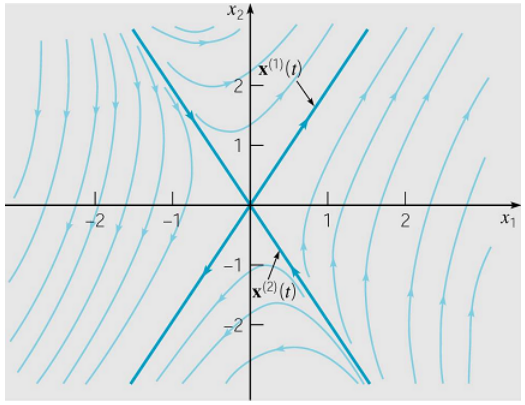
\includegraphics[width=0.45\textwidth]{figure/Lec12f2.PNG}
		\end{figure}
	\end{itemize}
	\textbf{Example 1: Phase plane for general solution (8 of 9)}
	\begin{figure}[H]
		\centering
			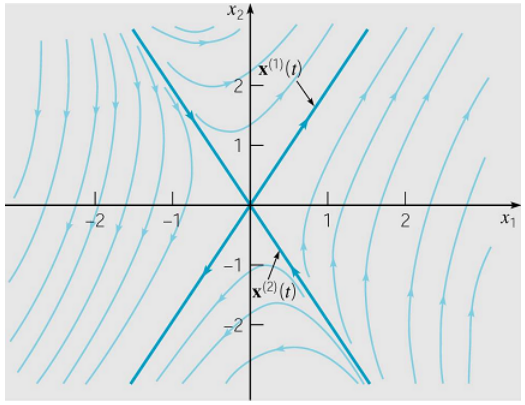
\includegraphics[width=0.55\textwidth]{figure/Lec12f2.PNG}
	\end{figure}
	\textbf{Example 1: Time plots for the general solution (9 of 9)}
	\begin{itemize}
		\item The general solution is $x = c_1x^{(1)} + c_2x^{(2)}$: 
		$$
		x(t) = c_1
		\begin{pmatrix}
			1\\
			2
		\end{pmatrix}e^{3t} + c_2
		\begin{pmatrix}
			1\\
			-2
		\end{pmatrix}\ \Leftrightarrow\ 
		\begin{pmatrix}
			x_1(t)\\
			x_2(t)
		\end{pmatrix}=
		\begin{pmatrix}
			c_1e^{3t} + c_2e^{-t}\\
			2c_1e^{3t} - 2c_2e^{-t}
		\end{pmatrix}
		$$
		\item As an alternative to phase plane plots, we can graph $x_1$ or $x_2$ as a function of $t$. A few plots of $x_1$ are given below. 
		\begin{figure}[H]
			\centering
				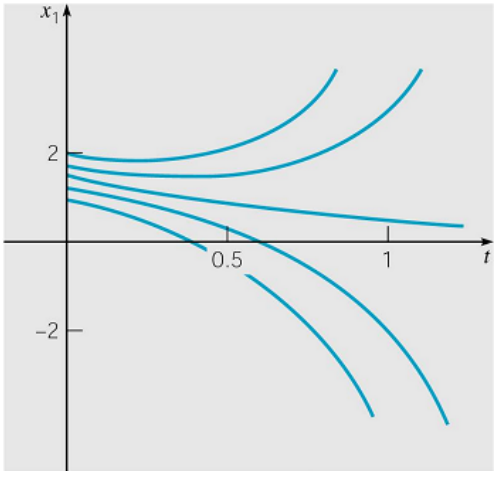
\includegraphics[width=0.45\textwidth]{figure/Lec12f3.PNG}
		\end{figure}
		\item Note that when $c_1 = 0,\ x_1(t) = c_2e^{-t}\to 0$ as $t \to \infty$. Otherwise, $x_1(t) = c_1e^{3t} + c_2e^{-t}$ grows unbounded as $t \to \infty$.
		\item Graphs of $x_2$ are similarly obtained.
	\end{itemize}
	\textbf{Example 1: Time plots for the general solution (9 of 9)}
	\begin{figure}[H]
		\centering
			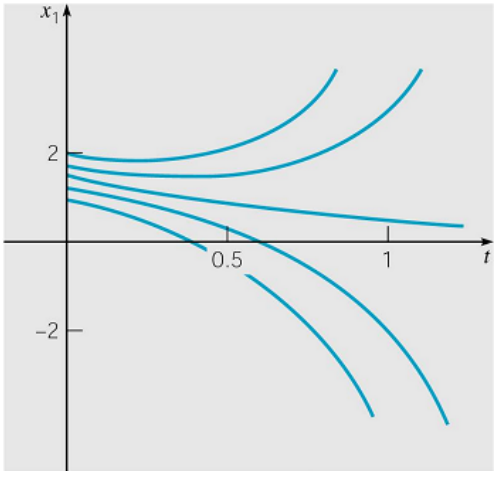
\includegraphics[width=0.55\textwidth]{figure/Lec12f3.PNG}
	\end{figure}
	%
	\textbf{Example 2: Direction field (1 of 9)}
	%
	\begin{itemize}
		\item Consider the homogeneous equation $x^\prime = Ax$ below.
		$$
		x^\prime =
		\begin{pmatrix}
			-2 & \sqrt{2}\\
			\sqrt{2} & -2
		\end{pmatrix}
		$$
		\item A direction field for this system is given below.
		%
		\begin{figure}[H]
			\centering
				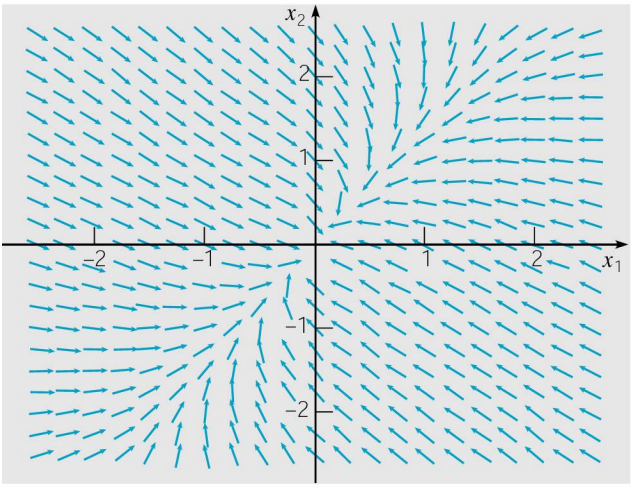
\includegraphics[width=0.45\textwidth]{figure/Lec12f4.PNG}
		\end{figure}
		%
		\item Substituting $x = \xi e^{rt}$ in for $x$, and rewriting the system as $(A-rI)\xi = 0$, we obtain
		$$
		\begin{pmatrix}
			-3-r & \sqrt{2}\\
			\sqrt{2} & -2-r
		\end{pmatrix}
		\begin{pmatrix}
			\xi_1\\
			\xi_2
		\end{pmatrix}=
		\begin{pmatrix}
			0\\
			0
		\end{pmatrix}
		$$ 
	\end{itemize}
	\textbf{Example 2: Eigenvalues (2 of 9) (brief)}
	\begin{itemize}
		\item Our solution has the form $x = \xi e^{rt}$, where $r$ and $\xi$ are found by solving
		$$
		\begin{pmatrix}
			-2-r & \sqrt{2}\\
			\sqrt{2} & -2-r
		\end{pmatrix}
		\begin{pmatrix}
			\xi_1\\
			\xi_2
		\end{pmatrix}=
		\begin{pmatrix}
			0\\
			0
		\end{pmatrix}
		$$
		\item Recalling that this is an eigenvalue problem, we determine $r$ by solving $\det(A-rI) = 0$:
		$$
		\begin{vmatrix}
			-3-r & \sqrt{2}\\
			\sqrt{2} & -2-r
		\end{vmatrix}=
		(-3-r)(-2-r)-2=r^2+5r+4=(r+1)(r+4)
		$$
		\item $r_1 = -1$ and $r_2 = -4$.
	\end{itemize}
	\textbf{Example 2: First eigenvector (3 of 9) (brief)}
	\begin{itemize}
		\item Eigenvector for $r_1 = -1$: Solve
		$$
		(A-rI)\xi = 0\ \Leftrightarrow\ 
		\begin{pmatrix}
			-3+1 & \sqrt{2}\\
			\sqrt{2} & -2+1
		\end{pmatrix}
		\begin{pmatrix}
			\xi_1\\
			\xi_2
		\end{pmatrix} =
		\begin{pmatrix}
			0\\
			0
		\end{pmatrix}\ \Leftrightarrow\ 
		\begin{pmatrix}
			-2 & \sqrt{2}\\
			\sqrt{2} & -1
		\end{pmatrix}
		\begin{pmatrix}
			\xi_1\\
			\xi_2
		\end{pmatrix}=
		\begin{pmatrix}
			0\\
			0
		\end{pmatrix}
		$$
		by row reducing the augmented matrix:\\
		$
		\begin{pmatrix}
			-2 & \sqrt{2} & 0\\
			\sqrt{2} & -1 & 0
		\end{pmatrix}\to
		\begin{pmatrix}
			1 & -\sqrt{2}/2 & 0\\
			\sqrt{2} & -1 & 0
		\end{pmatrix}\to
		\begin{pmatrix}
			1 & -\sqrt{2}/2 & 0\\
			0 & 0 & 0
		\end{pmatrix}\to
		\xi^{(1)} =
		\begin{pmatrix}
			\sqrt{2}/2\xi_2\\
			\xi_2
		\end{pmatrix}\to\ \text{chosse}\ \xi^{(1)} =
		\begin{pmatrix}
			1\\
			\sqrt{2}
		\end{pmatrix}
		$
	\end{itemize}
	\textbf{Example 2: Second eigenvector (4 of 9) (brief)}
	\begin{itemize}
		\item Eigenvector for $r_2 = -4$: Solve
		$$
		(A-rI) = 0\ \Leftrightarrow\ 
		\begin{pmatrix}
			-3+4 & \sqrt{2}\\
			\sqrt{2} & -2+4
		\end{pmatrix}
		\begin{pmatrix}
			\xi_1\\
			\xi_2
		\end{pmatrix}=
		\begin{pmatrix}
			0\\
			0
		\end{pmatrix}\ \Leftrightarrow\ 
		\begin{pmatrix}
			1 & \sqrt{2}\\
			\sqrt{2} & 2
		\end{pmatrix}
		\begin{pmatrix}
			\xi_1\\
			\xi_2
		\end{pmatrix}=
		\begin{pmatrix}
			0\\
			0
		\end{pmatrix}
		$$
		by row reducing the augmented matrix:\\
		$
		\begin{pmatrix}
			1 & \sqrt{2} & 0\\
			\sqrt{2} & 2 & 0
		\end{pmatrix}\to
		\begin{pmatrix}
			1 & \sqrt{2} & 0\\
			0 & 0 & 0
		\end{pmatrix}\to \xi^{(2)} =
		\begin{pmatrix}
			-\sqrt{2}\xi_2\\
			\xi_2
		\end{pmatrix}\to\ \text{choose}\ \xi^{(2)} =
		\begin{pmatrix}
			-\sqrt{2}\\
			1
		\end{pmatrix}
		$
	\end{itemize}
	\textbf{Example 2: General solution (5 of 9)}
	\begin{itemize}
		\item The corresponding solutions $x = \xi e^{rt}$ of $x^\prime = Ax$ are
		$$
		x^{(1)}(t)=
		\begin{pmatrix}
			1\\
			\frac{1}{\sqrt{2}}
		\end{pmatrix}e^{-t},\ 
		x^{(2)}(t) =
		\begin{pmatrix}
			-\sqrt{2}\\
			1
		\end{pmatrix}e^{-4t}
		$$
		\item The Wronskian of these two solutions is
		$$
		W[x^{(1)},x^{(2)}](t) =
		\begin{vmatrix}
			e^{-t} & -\sqrt{2}e^{-4t}\\
			\sqrt{2}e^{-t} & e^{-4t}
		\end{vmatrix} = 3e^{-5t} \neq 0
		$$
		\item Thus $x^{(1)}$ and $x^{(2)}$ are fundamental solutions, and the general solution of $x^\prime = Ax$ is
		\begin{align*}
			x(t) &= c_1x^{(1)}(t) + c_2x^{(2)}(t)\\
			&= c_1
			\begin{pmatrix}
				1\\
				\frac{1}{\sqrt{2}}
			\end{pmatrix}e^{-t} + c_2
			\begin{pmatrix}
				-\sqrt{2}\\
				1
			\end{pmatrix}e^{-4t}
		\end{align*}
	\end{itemize}
	\textbf{Example 2: Phase plane for $x^{(1)}$ (6 of 9) (brief)}
	\begin{itemize}
		\item To visualize the solution, consider first $x = c_1x^{(1)}$:
		$$
		x^{(1)}(t) =
		\begin{pmatrix}
			x_1\\
			x_2
		\end{pmatrix} = c_1
		\begin{pmatrix}
			1 \\
			\sqrt{2}
		\end{pmatrix}e^{-t}\ \Leftrightarrow\ 
		x_1 = c_1e^{-t},\ x_2 = \sqrt{2}c_1e^{-t}
		$$
		\item Now
		$$
		x_1 = c_1e^{-t},\ x_2 = \sqrt{2}c_1e^{-t}\ \Leftrightarrow\ e^{-t} = \frac{x_1}{c_1} = \frac{x_2}{\sqrt{2}c_1}\ \Leftrightarrow\ x_2 = \sqrt{2}x_1
		$$
		\item Thus $x^{(1)}$ lies along the straight line $x_2 = 2^{\nicefrac{1}{2}}x_1$, which is the line through origin in direction of first eigenvector $\xi^{(1)}$.
		\item If solution is trajectory of particle, with position given by $(x_1, x_2)$, then it is in Q1 when $c_1 > 0$, and in Q3 when $c_1 < 0$.
		\item In either case, a particle moves towards the origin as $t$ increases.
	\end{itemize}
	\textbf{Example 2: Phase plane for $x^{(2)}$ (7 of 9) (brief)}
	\begin{itemize}
		\item Next, consider $x = c_2x^{(2)}$:
		$$
		x^{(2)}(t) =
		\begin{pmatrix}
			x_1\\
			x_2
		\end{pmatrix}=c_2
		\begin{pmatrix}
			-\sqrt{2}\\
			1
		\end{pmatrix}e^{-4t}\ \Leftrightarrow\ x_1 = -\sqrt{2}c_2e^{-4t},\ x_2=c_2e^{-4t}
		$$
		\item Then $x^{(2)}$ lies along the straight line $x_2 = -2^{\nicefrac{1}{2}}x_1$, which is the line through the origin in the direction of the 2nd eigenvector $\xi^{(2)}$
		\item If the solution is the trajectory of a particle, with position given by $(x_1, x_2)$, then it is in Q4 when $c_2 > 0$, and in Q2 when $c_2 < 0$.
		\item In either case, the particle moves towards the origin as $t$ increases. 
	\end{itemize}
	\textbf{Example 2: Phase plane for the general solution (8 of 9)}
	\begin{itemize}
		\item The general solution is $x = c_1x^{(1)} + c_2x^{(2)}$:
		$$
		x^{(1)}(t) =
		\begin{pmatrix}
			1\\
			\sqrt{2}
		\end{pmatrix}e^{-t},\ x^{(2)}(t) =
		\begin{pmatrix}
			-\sqrt{2}\\
			1
		\end{pmatrix}e^{-4t}
		$$
		\item As $t\to \infty,\ c_1x^{(1)}$ is dominant and $c_2x^{(2)}$ becomes negligible. Thus, for $c_1 \neq 0$, all solutions asymptotically approach the origin along the line $x_2 = 2^{\nicefrac{1}{2}}x_1$ as $t\to \infty$.
		\item Similarly, all solutions are unbounded as $t \to -\infty$.
		\item The origin is a \textbf{node}, and is asymptotically stable.
		%
		\begin{figure}[H]
			\centering
				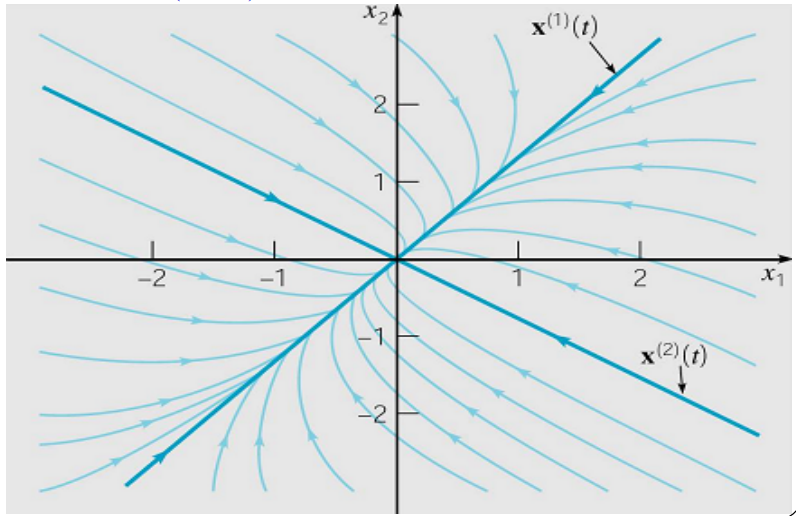
\includegraphics[width=0.45\textwidth]{figure/Lec12f5.PNG}
		\end{figure}
		%
	\end{itemize}
	\textbf{Example 2: Phase plane for the general solution (8 of 9)}
	%
	\begin{figure}[H]
		\centering
			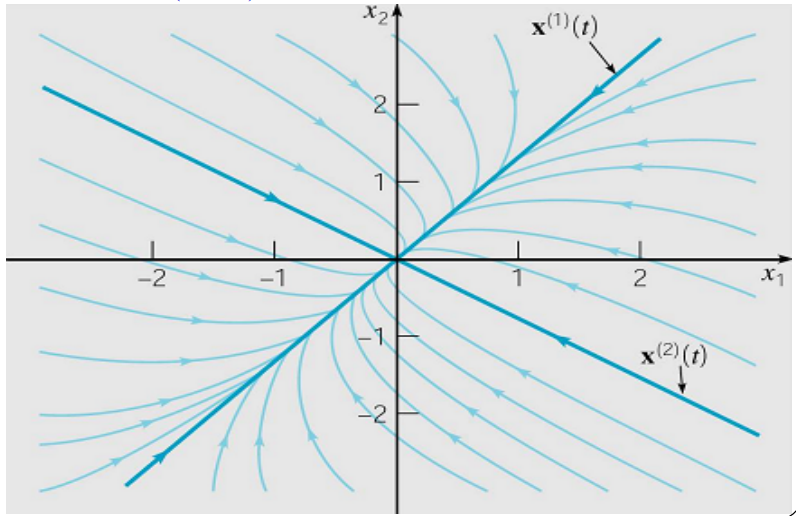
\includegraphics[width=0.55\textwidth]{figure/Lec12f5.PNG}
	\end{figure}
	%
	\textbf{Example 2: Time plots for the general solution (9 of 9)}
	\begin{itemize}
		\item The general solution is $x = c_1x^{(1)} + c_2x^{(2)}$:
		$$
		x(t)=c_1
		\begin{pmatrix}
			1\\
			\sqrt{2}e^{-t}
		\end{pmatrix}+c_2
		\begin{pmatrix}
			-\sqrt{2}\\
			1
		\end{pmatrix}e^{-4t}\ \Leftrightarrow\ 
		\begin{pmatrix}
			x_1(t)\\
			x_2(t)
		\end{pmatrix} =
		\begin{pmatrix}
			c_1e^{-t}-\sqrt{2}c_2e^{-4t}\\
			\sqrt{2}c_1e^{-t} + c_2e^{-4t}
		\end{pmatrix}
		$$
		\item As an alternative to phase plane plots, we can graph $x_1$ or $x_2$ as a function of $t$. A few plots of $x_1$ are given below.
		%
		\begin{figure}[H]
			\centering
				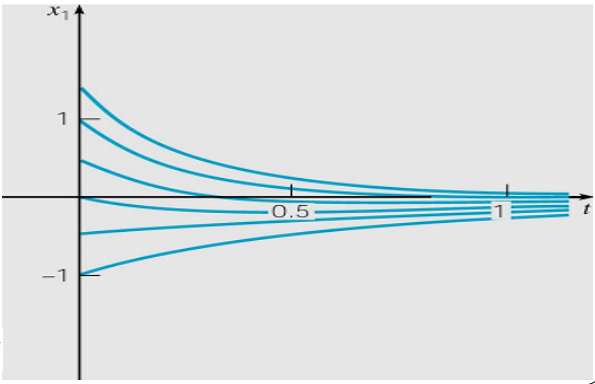
\includegraphics[width=0.45\textwidth]{figure/Lec12f6.PNG}
		\end{figure}
		%
		\item Graphs of $x_2$ are similarly obtained.
	\end{itemize}
	\textbf{Example 2: Time plots for the general solution (9 of 9)}
	%
	\begin{figure}[H]
		\centering
		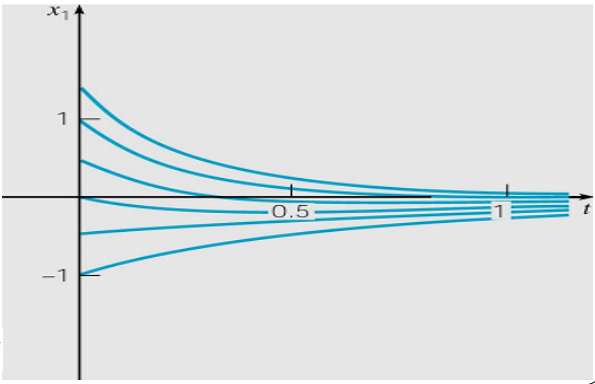
\includegraphics[width=0.55\textwidth]{figure/Lec12f6.PNG}
	\end{figure}
	%
	\textbf{$2 \times 2$ Case: Real eigenvalues, saddle points and nodes}
	\begin{itemize}
		\item The previous two examples demonstrate the two main cases for a $2 \times 2$ real system with real and different eigenvalues:
		\begin{itemize}
			\item[\labelitemi] Both eigenvalues have opposite signs, in which case origin is a saddle point and is unstable.
			\item[\labelitemi] Both eigenvalues have the same sign, in which case the origin is a node, and is asymptotically stable if the eigenvalues are negative and unstable if the eigenvalues are positive. 
		\end{itemize}
		%
		\begin{center}
			\begin{figure}[H]
				\centering
				\begin{subfigure}{.45\textwidth}
					\centering
					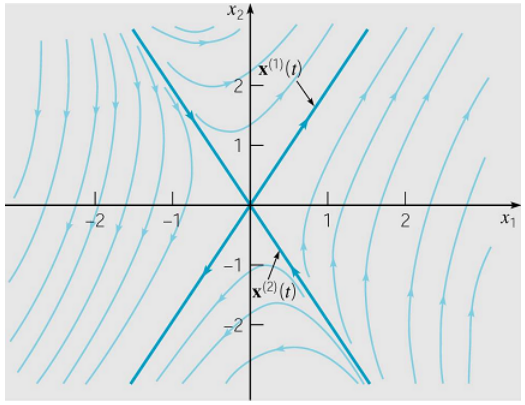
\includegraphics[width=0.75\textwidth]{figure/Lec12f2.PNG}
				\end{subfigure}
				%
				\begin{subfigure}{.45\textwidth}
					\centering
					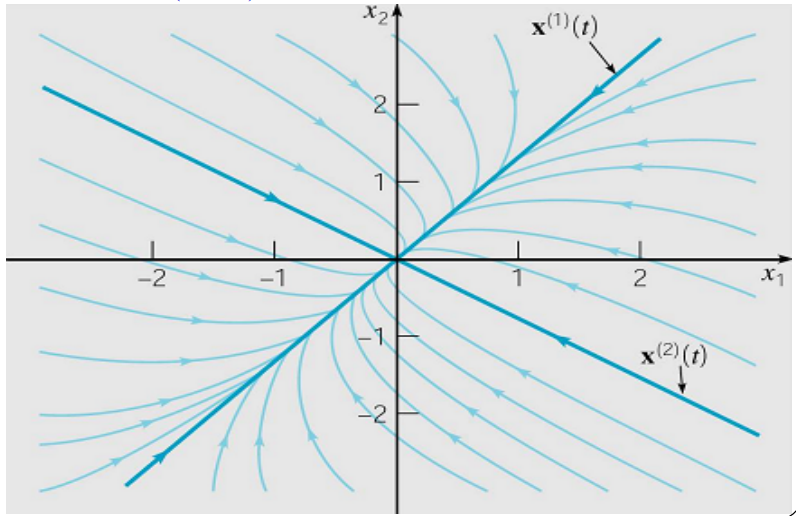
\includegraphics[width=0.87\textwidth]{figure/Lec12f5.PNG}
				\end{subfigure}
			\end{figure}
		\end{center}
		%
	\end{itemize}
	\textbf{Eigenvalues, eigenvectors and fundamental solutions}
	\begin{itemize}
		\item In general, for an $n \times n$ real linear system $x^\prime = Ax$:
		\begin{itemize}
			\item[\labelitemi] All eigenvalues are real and different from each other.
			\item[\labelitemi] Some eigenvalues are repeated.
			\item[\labelitemi] Some eigenvalues occur in complex conjugate pairs.
		\end{itemize}
		\item If eigenvalues $r_1,\ \ldots,\ r_n$ are real \& different, then there are $n$ corresponding linearly independent eigenvectors $\xi^{(1)},\ \ldots,\ \xi^{(n)}$.\\
		The associated solutions of $x^\prime = Ax$ are
		$$
		x^{(1)}(t) = \xi^{(1)}e^{r_1t},\ \ldots,\ \xi^{(n)}e^{r_nt}
		$$
		\item Using the Wronskian, it can be shown that these solutions are linearly independent, and hence form a fundamental set of solutions. Thus general solution is 
		$$
		x = c_1\xi^{(1)}e^{r_1t} + \ldots + c_n\xi^{(n)}e^{r_nt}
		$$
	\end{itemize}
	\textbf{Repeated Eigenvalues and Fundamental Solutions}
	\begin{itemize}
		\item If some of the eigenvalues $r_1,\ \ldots,\ r_n$ are repeated, then there may not be $n$ corresponding linearly independent solutions of the form
		$$
		x^{(1)}(t) = \xi^{(1)}e^{r_1t},\ \ldots,\ x^{(n)}(t) = \xi^{(n)}e^{r_nt}
		$$
		\item In order to obtain a fundamental set of solutions, it may be necessary to seek additional solutions of another form.
		\item This situation is analogous to that for an $n$th order linear equation with constant coefficients, in which case a repeated root gave rise to solutions of the form
		$$
		e^{rt},\ te^{rt},\ t^2e^{rt},\ \ldots
		$$
	\end{itemize}
\end{document}